\documentclass[]{article}
\usepackage[T1]{fontenc}
\usepackage{lmodern}
\usepackage{amssymb,amsmath}
\usepackage{ifxetex,ifluatex}
\usepackage{fixltx2e} % provides \textsubscript
% use upquote if available, for straight quotes in verbatim environments
\IfFileExists{upquote.sty}{\usepackage{upquote}}{}
\ifnum 0\ifxetex 1\fi\ifluatex 1\fi=0 % if pdftex
  \usepackage[utf8]{inputenc}
\else % if luatex or xelatex
  \ifxetex
    \usepackage{mathspec}
    \usepackage{xltxtra,xunicode}
  \else
    \usepackage{fontspec}
  \fi
  \defaultfontfeatures{Mapping=tex-text,Scale=MatchLowercase}
  \newcommand{\euro}{€}
\fi
% use microtype if available
\IfFileExists{microtype.sty}{\usepackage{microtype}}{}
\usepackage[margin=1in]{geometry}
\usepackage{longtable,booktabs}
\usepackage{graphicx}
% Redefine \includegraphics so that, unless explicit options are
% given, the image width will not exceed the width of the page.
% Images get their normal width if they fit onto the page, but
% are scaled down if they would overflow the margins.
\makeatletter
\def\ScaleIfNeeded{%
  \ifdim\Gin@nat@width>\linewidth
    \linewidth
  \else
    \Gin@nat@width
  \fi
}
\makeatother
\let\Oldincludegraphics\includegraphics
{%
 \catcode`\@=11\relax%
 \gdef\includegraphics{\@ifnextchar[{\Oldincludegraphics}{\Oldincludegraphics[width=\ScaleIfNeeded]}}%
}%
\ifxetex
  \usepackage[setpagesize=false, % page size defined by xetex
              unicode=false, % unicode breaks when used with xetex
              xetex]{hyperref}
\else
  \usepackage[unicode=true]{hyperref}
\fi
\hypersetup{breaklinks=true,
            bookmarks=true,
            pdfauthor={Sherri Verdugo},
            pdftitle={Chapter 8 Notes},
            colorlinks=true,
            citecolor=blue,
            urlcolor=blue,
            linkcolor=magenta,
            pdfborder={0 0 0}}
\urlstyle{same}  % don't use monospace font for urls
\setlength{\parindent}{0pt}
\setlength{\parskip}{6pt plus 2pt minus 1pt}
\setlength{\emergencystretch}{3em}  % prevent overfull lines
\setcounter{secnumdepth}{0}

%%% Change title format to be more compact
\usepackage{titling}
\setlength{\droptitle}{-2em}
  \title{Chapter 8 Notes}
  \pretitle{\vspace{\droptitle}\centering\huge}
  \posttitle{\par}
  \author{Sherri Verdugo}
  \preauthor{\centering\large\emph}
  \postauthor{\par}
  \predate{\centering\large\emph}
  \postdate{\par}
  \date{October 6, 2014}




\begin{document}

\maketitle


{
\hypersetup{linkcolor=black}
\setcounter{tocdepth}{3}
\tableofcontents
}
\subsection{Administration}\label{administration}

\begin{itemize}
\itemsep1pt\parskip0pt\parsep0pt
\item
  Attendance
\item
  Always read instructions for assignments:

  \begin{itemize}
  \itemsep1pt\parskip0pt\parsep0pt
  \item
    either in the forum, the initial posting, or the document itself
  \end{itemize}
\item
  Last Week:

  \begin{itemize}
  \itemsep1pt\parskip0pt\parsep0pt
  \item
    Chapter 7 Statistical Inference
  \end{itemize}
\item
  This Week: Inference at a Deeper Level
\item
  Chapter 8 Probability, z and t tests
\item
  Chapter 9 Two Sample t-tests
\item
  Today: Chapter 8 Probability Distributions
\item
  Upcoming Items

  \begin{itemize}
  \itemsep1pt\parskip0pt\parsep0pt
  \item
    Homework 2 released Monday 10/6/14
  \item
    Exam 2 10/22
  \item
    Writing Draft 10/29
  \end{itemize}
\end{itemize}

Feedback Packets (previous graded assignments and homework)

\subsection{Prologue \& Introduction}\label{prologue-introduction}

This chapter is a continuation of chapter 7. This chapter is focused on
what we are actually doing when we perform a $z$ test. Sometimes
understanding the underlying process, you gain more insight into the
task at hand. Case in point, taking care of a pool. You don't need to
understand the chemistry behind the chlorine and chemical test kits. If
you know it though, you have a better understanding of achieving a pool
that has appropriate levels of chlorine. Let's dive into statistics a
little bit further.

\subsection{Key Concepts}\label{key-concepts}

\begin{itemize}
\itemsep1pt\parskip0pt\parsep0pt
\item
  Normal Distribution

  \begin{itemize}
  \itemsep1pt\parskip0pt\parsep0pt
  \item
    A family of frequency distributions that, when graphed often
    resemble bells.
  \end{itemize}
\item
  Standard Score

  \begin{itemize}
  \itemsep1pt\parskip0pt\parsep0pt
  \item
    A score universally designated by the letter $z$, in which that
    score is expressed in standard deviation units from the mean.
  \end{itemize}
\item
  One-sample z Test

  \begin{itemize}
  \itemsep1pt\parskip0pt\parsep0pt
  \item
    A test of significance that can be performed when we know the
    population's standard deviation as well as its mean.
  \end{itemize}
\item
  Sampling Distribution of the Sample Means

  \begin{itemize}
  \itemsep1pt\parskip0pt\parsep0pt
  \item
    The frequency distribution that would be obtained from calculating
    the means of all theoretically possible samples of a designated size
    that could be drawn from a given population.
  \end{itemize}
\end{itemize}

\subsection{Key Concepts, continued}\label{key-concepts-continued}

\begin{itemize}
\itemsep1pt\parskip0pt\parsep0pt
\item
  Central Limit Theorem

  \begin{itemize}
  \itemsep1pt\parskip0pt\parsep0pt
  \item
    If repeated random samples of size n are drawn from a population
    that is normally distributed along some variable x, having a mean,
    $\mu$ and a standard deviation $\sigma$, the the sampling
    distribution of all theoretically possible sample means will be a
    normal distribution of all theoretically possible sample means will
    be a normal distribution having a mean $\mu$ and a standard
    deviation of $\frac{\sigma}{\sqrt{n}}$.
  \end{itemize}
\item
  Standard Error a.k.a. ``Standard Error of the Mean''

  \begin{itemize}
  \itemsep1pt\parskip0pt\parsep0pt
  \item
    The standard deviation of the sampling distribution, designated with
    the symbol $\sigma_{\bar{x}}$
  \end{itemize}
\item
  Normality Assumption

  \begin{itemize}
  \itemsep1pt\parskip0pt\parsep0pt
  \item
    The assumption that the population being studied is normally
    distributed along variable x.
  \end{itemize}
\item
  Law of Large Numbers

  \begin{itemize}
  \itemsep1pt\parskip0pt\parsep0pt
  \item
    A law that states that if the size of the sample, $n$, is
    sufficiently large (no less than 30, preferably no less than 50),
    then the Central Limit Theorem will apply even if the population is
    not normally distributed along, variable x.
  \end{itemize}
\end{itemize}

\textbf{Note: this requires further testing in the real world\ldots{}for
this class, we will use that assumption without testing. However, we may
find ourselves in the real world testing the normality of a distribution
along a variable x.}

\subsection{Key Concepts, continued}\label{key-concepts-continued-1}

\begin{itemize}
\itemsep1pt\parskip0pt\parsep0pt
\item
  ``sigma-hat'' $\hat{\sigma}$

  \begin{itemize}
  \itemsep1pt\parskip0pt\parsep0pt
  \item
    An estimate of sigma. Note: if you see anything with a hat on
    it\ldots{}we are using an ESTIMATE.
  \end{itemize}
\item
  t Test

  \begin{itemize}
  \itemsep1pt\parskip0pt\parsep0pt
  \item
    A test of significance similar to the z test but used when the
    population's standard deviation is unknown.
  \end{itemize}
\item
  Degrees of Freedom

  \begin{itemize}
  \itemsep1pt\parskip0pt\parsep0pt
  \item
    A number that is generated to make use of a table of critical
    values. It is the number of values in the final calculation of a
    statistic that are free to vary.
  \end{itemize}
\end{itemize}

\subsection{Key Concepts, continued}\label{key-concepts-continued-2}

\begin{itemize}
\itemsep1pt\parskip0pt\parsep0pt
\item
  z Test for Proportions

  \begin{itemize}
  \itemsep1pt\parskip0pt\parsep0pt
  \item
    A z test designed to test whether the difference between proportions
    in a sample reflects the difference in the population.
  \end{itemize}
\item
  Interval Estimation

  \begin{itemize}
  \itemsep1pt\parskip0pt\parsep0pt
  \item
    An interval of scores that is established, within which a
    population's mean (or another parameter is likely to fall, when that
    parameter is being estimated from sample data).
  \end{itemize}
\item
  Confidence Intervals for Means and Proportions

  \begin{itemize}
  \itemsep1pt\parskip0pt\parsep0pt
  \item
    An estimated interval within which we are ``confident'' -- based on
    sampling theory -- that the parameter we are trying to estimate will
    fall.
  \end{itemize}
\end{itemize}

\subsection{Key Concepts, continued}\label{key-concepts-continued-3}

\begin{itemize}
\itemsep1pt\parskip0pt\parsep0pt
\item
  Conditional Probability

  \begin{itemize}
  \itemsep1pt\parskip0pt\parsep0pt
  \item
    The probability of outcome $A$ occurring given that the outcome for
    $B$ has already occurred.
  \end{itemize}
\item
  Addition Rules of Probability

  \begin{itemize}
  \itemsep1pt\parskip0pt\parsep0pt
  \item
    A rule by which when outcomes are \textbf{MUTUALLY EXCLUSIVE}, the
    probability of either outcome occurring is the sum of the
    probabilities of each outcome occurring.
  \end{itemize}
\item
  Multiplication Rules of Probability

  \begin{itemize}
  \itemsep1pt\parskip0pt\parsep0pt
  \item
    A rule that is used to find $P(A and D)$.
  \end{itemize}
\item
  Permutations

  \begin{itemize}
  \itemsep1pt\parskip0pt\parsep0pt
  \item
    The total possible samples that can be drawn from a population where
    the order of selection is a factor.
  \end{itemize}
\item
  Combinations

  \begin{itemize}
  \itemsep1pt\parskip0pt\parsep0pt
  \item
    The total possible samples when the order of selection is ignored.
  \end{itemize}
\end{itemize}

\subsection{Chapter 8 Outline}\label{chapter-8-outline}

\begin{itemize}
\itemsep1pt\parskip0pt\parsep0pt
\item
  Introduction
\item
  Normal Distributions
\item
  Proportion of Area Under Standard Normal Curves
\item
  One Sample $z$ Test for Statistical Significance
\item
  Central Limit Theorem
\item
  CLT and Hypothesis Testing Review
\item
  Normality Assumption
\item
  One Sample t-test for Statistical Inference
\item
  Degrees of Freedom
\item
  The t Table
\item
  Alternative t Formula
\item
  A z Test for Proportions
\item
  Interval Estimation
\item
  Confidence Intervals for Proportions
\item
  A FEW MORE WORDS ON PROBABILITY
\item
  Permutations and Combinations
\item
  Conclusion
\item
  Major Equations for Chapter 8
\end{itemize}

\subsection{Introduction}\label{introduction}

\begin{itemize}
\itemsep1pt\parskip0pt\parsep0pt
\item
  Chapter 7 introduced the test of significance under the lens of the
  $z$ score to demonstrate the procedure. Recall, that
  $z = \frac{\bar{x} - \mu}{\frac{\sigma}{\sqrt{n}}}$.
\item
  Characteristics of $z$

  \begin{itemize}
  \itemsep1pt\parskip0pt\parsep0pt
  \item
    Frequency distribution: normal distribution
  \item
    Applied to a specific normal curve: sampling distribution of the
    sample means.
  \end{itemize}
\item
  What are we doing with $z$

  \begin{itemize}
  \itemsep1pt\parskip0pt\parsep0pt
  \item
    Taking the given sample statistic and population parameters
  \item
    Locating them on the sampling distribution of the sample means
  \end{itemize}
\item
  All significance tests follow the same method. They just use different
  sampling distributions.
\item
  The test you use must be appropriate for the distribution!
\end{itemize}

\subsection{Normal Distributions}\label{normal-distributions}

\subsubsection{What is normal?}\label{what-is-normal}

\begin{itemize}
\itemsep1pt\parskip0pt\parsep0pt
\item
  Normal is a family of frequency distributions that, when graphed often
  resemble bells.
\item
  Normal = Gaussian
\end{itemize}

\subsubsection{Family of gaussian distrubutions, by increasing st.
deviation 1 to
4}\label{family-of-gaussian-distrubutions-by-increasing-st.-deviation-1-to-4}

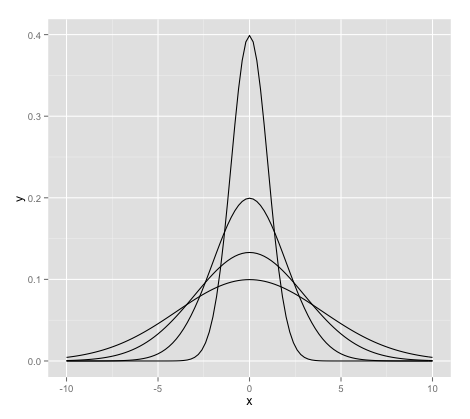
\includegraphics{normal.png}

\subsection{Normal Distributions,
continued}\label{normal-distributions-continued}

\subsubsection{Major characteristics}\label{major-characteristics}

\begin{itemize}
\itemsep1pt\parskip0pt\parsep0pt
\item
  uni modal
\item
  symmetric
\item
  asymptotic to the x-axis
\end{itemize}

\subsubsection{Reason for the term
``normal''}\label{reason-for-the-term-normal}

\begin{itemize}
\itemsep1pt\parskip0pt\parsep0pt
\item
  certain characteristics follow a normal distribution

  \begin{itemize}
  \itemsep1pt\parskip0pt\parsep0pt
  \item
    height
  \item
    weight
  \item
    intelligence
  \end{itemize}
\item
  Not everything in nature is normally distributed.
\item
  Other distributions are not ``abnormal''\ldots{}they are just
  ``different distributions''
\end{itemize}

\subsection{Normal Distributions: Standard
Scores}\label{normal-distributions-standard-scores}

\begin{itemize}
\itemsep1pt\parskip0pt\parsep0pt
\item
  Standard Score

  \begin{itemize}
  \itemsep1pt\parskip0pt\parsep0pt
  \item
    score that is universally designated by the letter $z$, in which
    that score is expressed in standard deviation units from the mean.
  \end{itemize}
\end{itemize}

This time our equation is this: $\frac{x-\mu}{\sigma}$ and the table for
proportions of area under the standard normal curve is

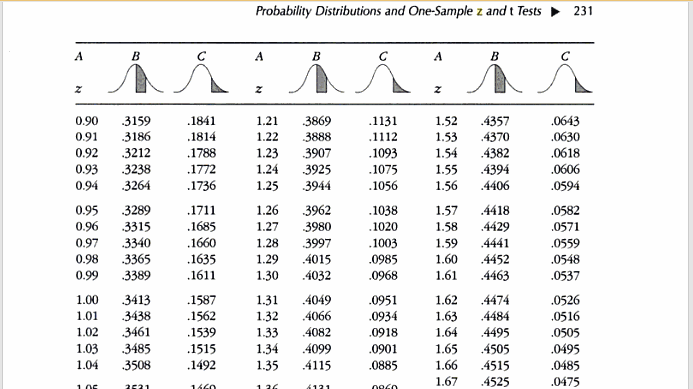
\includegraphics{ztable.png}

\subsubsection{How do we read this
table?}\label{how-do-we-read-this-table}

\subsection{Reading the table for proportions of area under the standard
normal
curve}\label{reading-the-table-for-proportions-of-area-under-the-standard-normal-curve}

\begin{itemize}
\itemsep1pt\parskip0pt\parsep0pt
\item
  On the previous slide, we saw a portion of the table for proportions
  of area under the standard normal curve.
\item
  Steps to read the table

  \begin{itemize}
  \itemsep1pt\parskip0pt\parsep0pt
  \item
    Three columns of A: these are the values of $z$ calculated from the
    equation
  \item
    Three columns of B: these are the area under the curve from the mean
    \emph{out to the specified value of z}
  \item
    Three columns of C: these are the area in the tail \emph{from} the z
    score (the tails)
  \end{itemize}
\item
  Tip: the area from column B and column C add to .50 or 50\%

  \begin{itemize}
  \itemsep1pt\parskip0pt\parsep0pt
  \item
    Example: z = 0.17 with Column B = 0.0675 and Column C = 0.4325 so,
  \item
    $0.0675 + 0.4325 = 0.5000$ or 50\%
  \end{itemize}
\item
  Tip: as z get larger

  \begin{itemize}
  \itemsep1pt\parskip0pt\parsep0pt
  \item
    Column B gets larger
  \item
    Column C gets SMALLER
  \end{itemize}
\end{itemize}

\subsection{Z Score example with the table pages 227 to
230}\label{z-score-example-with-the-table-pages-227-to-230}

\subsubsection{Sandy's IQ}\label{sandys-iq}

Question: What proportion of people are above and below Sandy's IQ.

\begin{itemize}
\itemsep1pt\parskip0pt\parsep0pt
\item
  Sandy score = 115 (observed)
\item
  Mean = 100 (expected)
\item
  Standard Deviation is 10
\end{itemize}

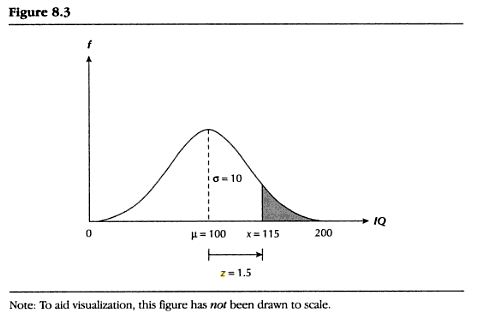
\includegraphics{sandy1.png}

\subsubsection{So how do we handle
this?}\label{so-how-do-we-handle-this}

\subsection{Sandy's z Score}\label{sandys-z-score}

The z equation is: $\frac{x - \mu}{\sigma}$

\begin{itemize}
\itemsep1pt\parskip0pt\parsep0pt
\item
  Sandy's z score is: $\frac{115 - 100}{10}=\frac{15}{10}=1.5$
\end{itemize}

\subsubsection{From the z table in the
book:}\label{from-the-z-table-in-the-book}

\begin{itemize}
\itemsep1pt\parskip0pt\parsep0pt
\item
  Percentage of people below Sandy

  \begin{itemize}
  \itemsep1pt\parskip0pt\parsep0pt
  \item
    IQs between 100 and 114 for $z=1.5$ (column B) = .4332
  \item
    IQs between 0 and 100: = .5000 (50 percent of the people are below
    the population mean or expected mean)
  \item
    Add these two together: $.4332 + .500 = .9332$, which is the
    proportion of people with IQs below Sandy! Pretty Smart, eh? Sandy
    is above the mean (that is why the z score is positive).
  \end{itemize}
\end{itemize}

\subsubsection{The proportion of people with IQs below Sandy is
.9332}\label{the-proportion-of-people-with-iqs-below-sandy-is-.9332}

\subsection{What about when z is negative? Pg.
229}\label{what-about-when-z-is-negative-pg.-229}

What if George has a score of 80 on the IQ? This is not a problem
because we know z scores can be positive (above the mean) and negative
(below the mean).

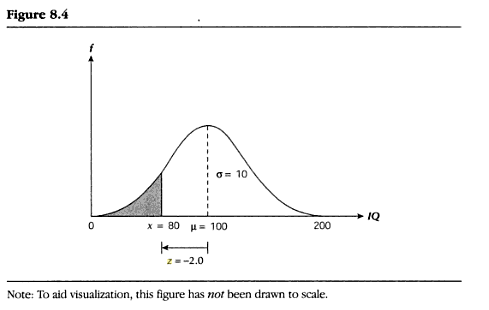
\includegraphics{george1.png}

\begin{itemize}
\itemsep1pt\parskip0pt\parsep0pt
\item
  George's z score is: $\frac{80 - 100}{10}=\frac{-20}{10}=-2.0$
\item
  At first, you might be confused\ldots{}but remember that the normal
  curve is symmetrical.

  \begin{itemize}
  \itemsep1pt\parskip0pt\parsep0pt
  \item
    Meaning what happens on one side of the mean will happen on the
    other side of the mean\ldots{}you can use z = 2.00 on page 232 of
    the textbook.
  \item
    Column B is .4772
  \item
    \textbf{Column C is .0228} the proportion of people with IQs below
    George
  \end{itemize}
\item
  We are still not finished with the proportion of people \textbf{Above}
  George.

  \begin{itemize}
  \itemsep1pt\parskip0pt\parsep0pt
  \item
    Recall that .5000 are above the mean (properties of the st. normal
    curve)\ldots{}and we need the proportion from George's score to the
    mean.
  \item
    Therefore $.4772 + 0.500 = 0.9772$
  \end{itemize}
\end{itemize}

\subsubsection{Nearly 98\% of all IQ scores fall above George's
score.}\label{nearly-98-of-all-iq-scores-fall-above-georges-score.}

\subsection{One Sample z Test for Statistical Significance: One
Tail}\label{one-sample-z-test-for-statistical-significance-one-tail}

\subsubsection{Chapter 7 Equation for z}\label{chapter-7-equation-for-z}

\begin{itemize}
\itemsep1pt\parskip0pt\parsep0pt
\item
  Used for the following frequency distribution:

  \begin{itemize}
  \itemsep1pt\parskip0pt\parsep0pt
  \item
    Sampling distribution of sample means
  \end{itemize}
\item
  Equation: $z = \frac{\bar{x}-\mu}{\frac{\sigma}{sqrt{n}}}$
\item
  One Tail Critical Values of z

  \begin{itemize}
  \itemsep1pt\parskip0pt\parsep0pt
  \item
    in this case we are looking at positive values (above the mean)
  \item
    this applies to the negative values (below the mean)
    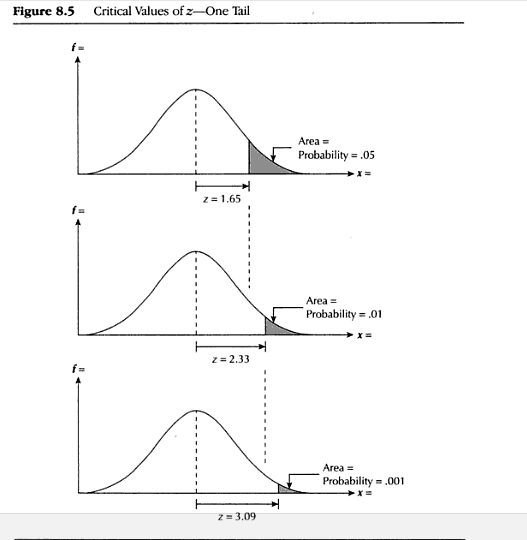
\includegraphics{z1tail.png}
  \end{itemize}
\item
  Sampling Distribution of Sample Means: frequency distribution that
  would be obtained from calculating the means of all theoretically
  possible sample of a designated size that could be drawn from a
  population.
\end{itemize}

\subsection{One Sample z Test for Statistical Significance: Two
Tail}\label{one-sample-z-test-for-statistical-significance-two-tail}

\begin{itemize}
\itemsep1pt\parskip0pt\parsep0pt
\item
  Used for the following frequency distribution:

  \begin{itemize}
  \itemsep1pt\parskip0pt\parsep0pt
  \item
    Sampling distribution of sample means
    $z = \frac{\bar{x}-\mu}{\frac{\sigma}{sqrt{n}}}$
  \end{itemize}
\item
  Two Tail Critical Values of z 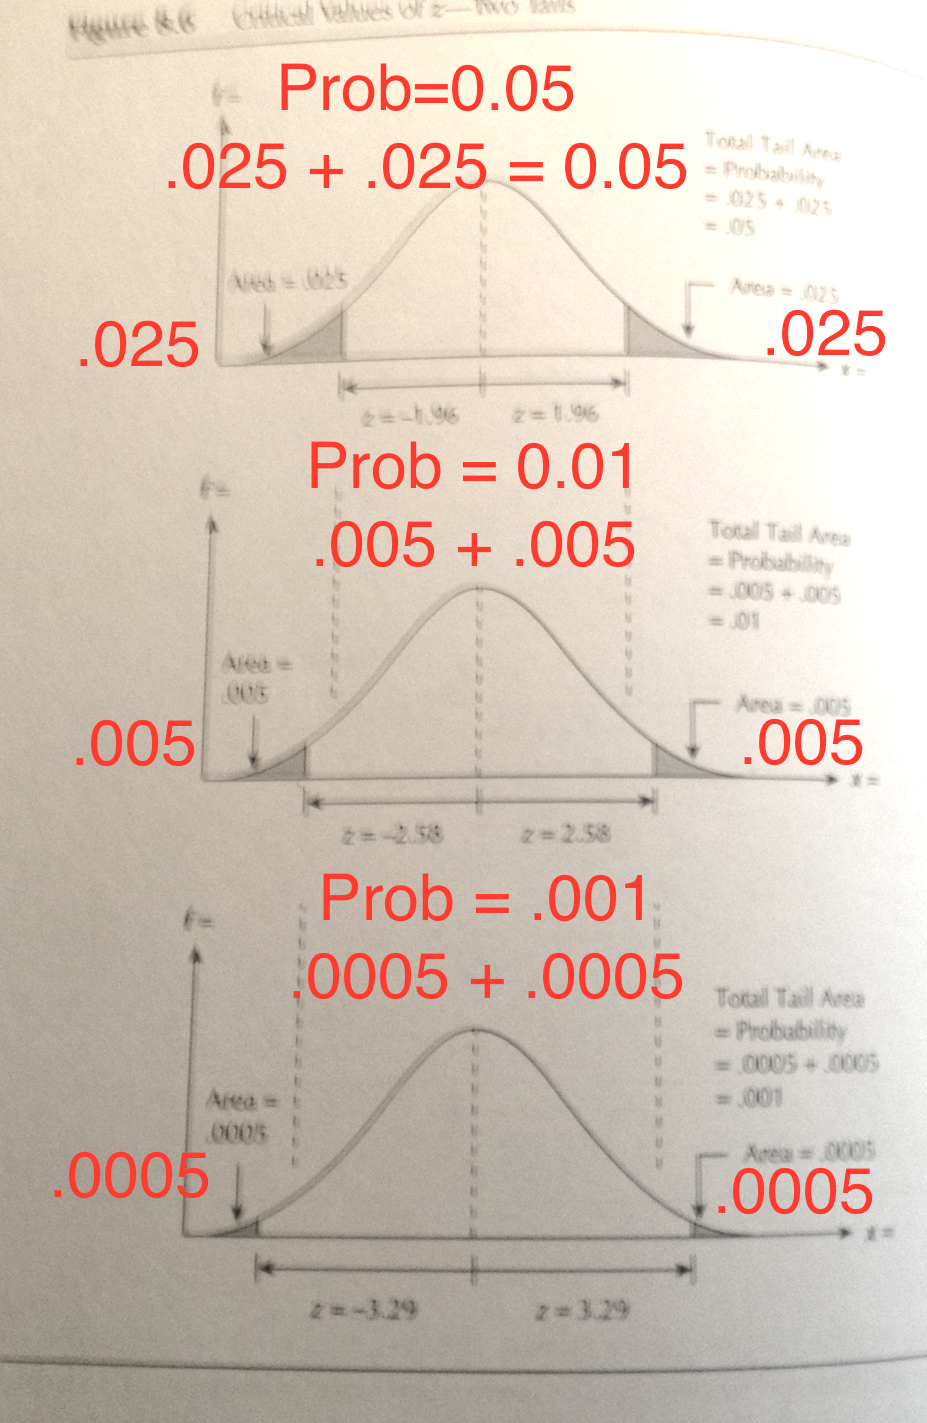
\includegraphics{z2tails.png}
\item
  Sampling Distribution of Sample Means: frequency distribution that
  would be obtained from calculating the means of all theoretically
  possible sample of a designated size that could be drawn from a
  population.
\end{itemize}

\subsection{Working out the sampling distribution of the
mean}\label{working-out-the-sampling-distribution-of-the-mean}

\begin{itemize}
\itemsep1pt\parskip0pt\parsep0pt
\item
  Scores range from: 1 to 5 \ldots{}. (i.e.~1,2,3,4,5)
\item
  Sample size, $n = 3$
\item
  To find the different combinations of 10 samples using n=3
\end{itemize}

\begin{longtable}[c]{@{}lllllllllll@{}}
\toprule\addlinespace
test & x1 = & x2 = & x3 = & x4 = & x5 = & x6 = & x7 = & x8 = & x9 = &
x10 =
\\\addlinespace
\midrule\endhead
1 & 5 & 5 & 5 & 5 & 5 & 5 & 4 & 4 & 4 & 3
\\\addlinespace
2 & 4 & 4 & 4 & 3 & 3 & 2 & 3 & 3 & 3 & 2
\\\addlinespace
3 & 3 & 2 & 1 & 2 & 1 & 1 & 2 & 1 & 1 & 1
\\\addlinespace
$\Sigma$ & \emph{12} & \emph{11} & \emph{10} & \emph{10} & \emph{9} &
\emph{8} & \emph{9} & \emph{8} & \emph{8} & \emph{6}
\\\addlinespace
$\bar{x}$ & \textbf{4} & \textbf{3.7} & \textbf{3.3} & \textbf{3.3} &
\textbf{3} & \textbf{2.7} & \textbf{3} & \textbf{2.7} & \textbf{2.7} &
\textbf{2}
\\\addlinespace
\bottomrule
\end{longtable}

\begin{itemize}
\itemsep1pt\parskip0pt\parsep0pt
\item
  $\bar{x}=\frac{\sigma x}{3}$
\end{itemize}

$\bar{x}$ Values and Frequencies

\begin{longtable}[c]{@{}llllllll@{}}
\toprule\addlinespace
$\bar{x}$ & 4.0 & 3.7 & 3.3 & 3.0 & 2.7 & 2.3 & 2.0
\\\addlinespace
\midrule\endhead
$f$ & 1 & 1 & 2 & 2 & 2 & 1 & 1
\\\addlinespace
\bottomrule
\end{longtable}

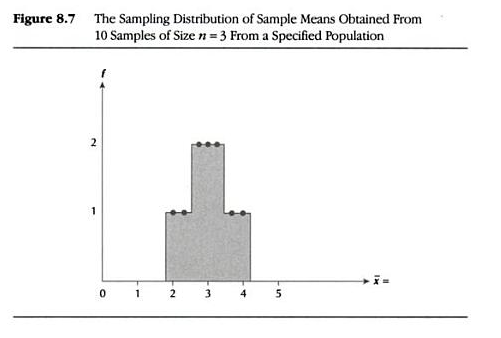
\includegraphics{x_bar1.png}

\begin{itemize}
\itemsep1pt\parskip0pt\parsep0pt
\item
  Formal Reason behind this: \emph{Central Limit Theorem} \& the
  \emph{Law of Large Numbers}
\end{itemize}

\subsection{The FAMOUS \& FABULOUS Central Limit Theorem
(CLT)}\label{the-famous-fabulous-central-limit-theorem-clt}

\textbf{CLT}: If repeated random samples of size n are drawn from a
population that is normally distributed along some variable x, having a
mean, $\mu$ and a standard deviation $\sigma$, the the sampling
distribution of all theoretically possible sample means will be a normal
distribution of all theoretically possible sample means will be a normal
distribution having a mean $\mu$ and a standard deviation of
$\frac{\sigma}{\sqrt{n}}$.

\begin{itemize}
\item
  For a particular population, a variable (x) is normally distributed
  \ldots{} if we draw a series of samples of predetermined approximately
  large sample size (n) from that population, the CLT tells us the
  following:
\item
  Sampling distribution of sample means will be a NORMAL DISTRIBUTION
\item
  The mean of the sampling distribution of sample means:

  \begin{itemize}
  \itemsep1pt\parskip0pt\parsep0pt
  \item
    the mean of all sample means (designated $\bar{x}$) will be EQUAL TO
    $\mu$
  \item
    $\mu$ is the mean from the population that the sample is drawn from.
  \end{itemize}
\item
  The St.~Dev. of the sampling distribution of sample means

  \begin{itemize}
  \itemsep1pt\parskip0pt\parsep0pt
  \item
    will be EQUAL to $\frac{\sigma}{n}$
  \item
    new concept \emph{Standard Error of the Mean} or \emph{SEM}
  \end{itemize}
\end{itemize}

\subsubsection{Standard Error of the
Mean}\label{standard-error-of-the-mean}

The standard deviation of the sampling distribution, designated with the
symbol $\sigma_{\bar{x}}$

\subsection{CLT graphically}\label{clt-graphically}

Histogram with, n=100, $\mu=70$ and $\sigma=20$

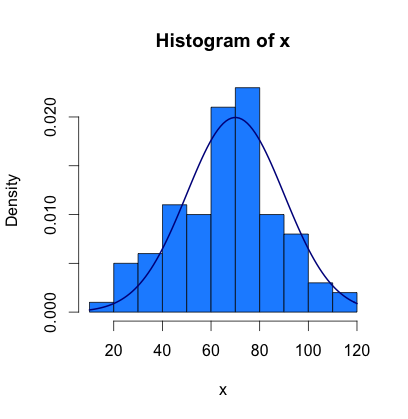
\includegraphics{hist2.png}

From the text book, the actual appearance of a sampling distribution

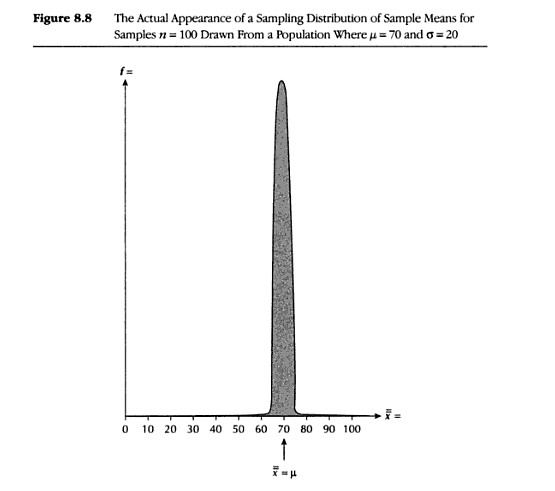
\includegraphics{clt1.png}

\begin{longtable}[c]{@{}lll@{}}
\toprule\addlinespace
Possible Sample Means \% & Range from Mean (in st. errors) & Range in
Exam Scores
\\\addlinespace
\midrule\endhead
68.27\% & $\mu \pm 1 \sigma_{\bar{x}}$ & 68-72
\\\addlinespace
95.45\% & $\mu \pm 2 \sigma_{\bar{x}}$ & 66-74
\\\addlinespace
99.73\$ & $\mu \pm 3 \sigma_{\bar{x}}$ & 64-76
\\\addlinespace
\bottomrule
\end{longtable}

\subsubsection{Area under the normal curve = percentage of all possible
sample
means}\label{area-under-the-normal-curve-percentage-of-all-possible-sample-means}

\subsection{CLT at work\ldots{}.an example through a
story}\label{clt-at-work.an-example-through-a-story}

Scenario: A competency exam score is given to students with a sample
size of 100 ninth grade students enrolled in a six week course to
prepare for the exam. The sample mean is 73, the population mean is 70,
and the population standard deviation is 20. Set alpha to .05 and use a
one-tailed directional hypothesis.

\subsubsection{Hypothesis}\label{hypothesis}

\begin{itemize}
\itemsep1pt\parskip0pt\parsep0pt
\item
  Null -- $H_0: \mu_{all} = \mu_{course}$
\item
  Directional Alt -- $H_1: \mu_{all} ≠ \mu_{course}$
\end{itemize}

\subsubsection{Equation for z using chapter
7}\label{equation-for-z-using-chapter-7}

$z = \frac{\bar{x}-\mu}{\frac{\sigma}{\sqrt{n}}}$

\subsubsection{Plugging in from our story problem and
solving}\label{plugging-in-from-our-story-problem-and-solving}

$z = \frac{73-70}{\frac{20}{\sqrt{100}}}$ and
$\frac{3}{\frac{20}{\sqrt{100}}}$ = $\frac{3}{\frac{20}{10}}$ =
$\frac{3}{2}$ = 1.50

\subsubsection{Significant or not\ldots{}}\label{significant-or-not}

Critical value of z when $\alpha=0.05$ is 1.65 and we reject if our z is
greater. Drum roll\ldots{}.the result is: $1.50 < 1.65$ and we
\textbf{fail} to reject $H_0$ in favor of the $H_1$

\subsection{Normality Assumption}\label{normality-assumption}

The assumption that the population being studied is normally distributed
along variable x.

\subsection{Law of Large Numbers}\label{law-of-large-numbers}

A law that states that if the size of the sample, $n$, is sufficiently
large (no less than 30, preferably no less than 50), then the Central
Limit Theorem will apply even if the population is not normally
distributed along, variable x.

\subsubsection{Rules for N}\label{rules-for-n}

\begin{longtable}[c]{@{}ll@{}}
\toprule\addlinespace
$IF$ & $THEN$
\\\addlinespace
\midrule\endhead
$n ≥ 100$ & It is always safe to relax the normality assumption (for
this class)
\\\addlinespace
$50≤n≤100$ & It is \emph{ALMOST} always safe to relax the normality
assumption
\\\addlinespace
$30≤n≤50$ & It is \emph{PROBABLY} safe to relax the normality assumption
\\\addlinespace
$n < 30$ & It is \emph{PROBABLY} \textbf{NOT} safe to relax the
normality assumption
\\\addlinespace
\bottomrule
\end{longtable}

\subsection{A last little bit on Z}\label{a-last-little-bit-on-z}

For $z$ we have to know population parameters, $\mu$ and $\sigma$

Let's dissect the following graph

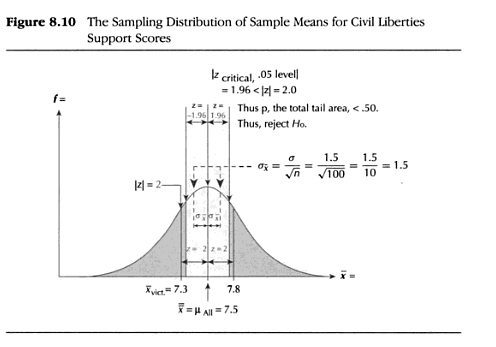
\includegraphics{one_samp_z_clib.png}

\begin{itemize}
\item
  We reject the $H_0$ when $p < .05$
\item
  We would retain the $H_0$ when $p > .05$
\item
  $z$ is ALWAYS NORMAL!
\end{itemize}

\subsection{One Sample t-test for Statistical
Inference}\label{one-sample-t-test-for-statistical-inference}

\subsubsection{Variance revisited}\label{variance-revisited}

This is a new version of the standard deviation equation, but recall the
equation for standard deviation which is the square root of variance. It
is really this equation: $\sqrt{\frac{\Sigma (x-\bar{x})^2}{n}}$.

\subsubsection{The t- test}\label{the-t--test}

\begin{itemize}
\itemsep1pt\parskip0pt\parsep0pt
\item
  First, we need a way to estimate $\sigma$ and we do this by placing a
  ``hat'' on sigma. $\hat{sigma}$

  \begin{itemize}
  \itemsep1pt\parskip0pt\parsep0pt
  \item
    $\hat{\sigma} = \sqrt{\frac{\Sigma (x - \bar{x})^2}{n-1}}$
  \end{itemize}
\item
  The equation for t-test:
  $t=\frac{\bar{x}-\mu}{\frac{\hat{\sigma}}{\sqrt{n}}}$
\item
  t Test: a test of significance similar to the $z$ test but used when
  the population's standard deviation is \textbf{unknown}.
\item
  t is \textbf{NOT} ALWAYS normal.
\end{itemize}

\subsection{Changes in the Sampling Distribution of t as Sample Size
Decreases}\label{changes-in-the-sampling-distribution-of-t-as-sample-size-decreases}

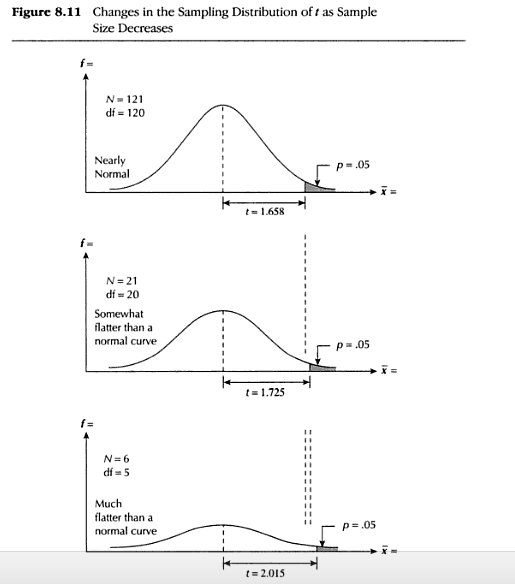
\includegraphics{t_dist1.png}

\subsection{Degrees of Freedom (a.k.a.
``DF'')}\label{degrees-of-freedom-a.k.a.-df}

\begin{itemize}
\itemsep1pt\parskip0pt\parsep0pt
\item
  In the figure on the previous slide, we introduced a new
  concept\ldots{}DF
\item
  Textbook definition of Degrees of Freedom:

  \begin{itemize}
  \itemsep1pt\parskip0pt\parsep0pt
  \item
    A number that is generated to make use of a table of critical values
  \end{itemize}
\item
  It is the number of independent ways by which a dynamic system can
  move without violating any constraint imposed on it, is called degree
  of freedom. In other words, the degree of freedom can be defined as
  the minimum number of independent coordinates that can specify the
  position of the system completely.
\item
  Estimates of statistical parameters can be based upon different
  amounts of information or data. The number of independent pieces of
  information that go into the estimate of a parameter is called the
  degrees of freedom. In general, the degrees of freedom of an estimate
  of a parameter is equal to the number of independent scores that go
  into the estimate minus the number of parameters used as intermediate
  steps in the estimation of the parameter itself (i.e., the sample
  variance has N-1 degrees of freedom, since it is computed from N
  random scores minus the only 1 parameter estimated as intermediate
  step, which is the sample mean).
\item
  Mathematically, degrees of freedom is the number of dimensions of the
  domain of a random vector, or essentially the number of `free'
  components (how many components need to be known before the vector is
  fully determined).
\item
  The term is most often used in the context of linear models (linear
  regression, analysis of variance), where certain random vectors are
  constrained to lie in linear sub spaces, and the number of degrees of
  freedom is the dimension of the subspace. The degrees of freedom are
  also commonly associated with the squared lengths (or ``sum of
  squares'' of the coordinates) of such vectors, and the parameters of
  chi-squared and other distributions that arise in associated
  statistical testing problems.
\item
  While introductory textbooks may introduce degrees of freedom as
  distribution parameters or through hypothesis testing, it is the
  underlying geometry that defines degrees of freedom, and is critical
  to a proper understanding of the concept. Walker (1940) has stated
  this succinctly as ``the number of observations minus the number of
  necessary relations among these observations.''
\end{itemize}

\subsubsection{Source:
\url{http://en.wikipedia.org/wiki/Degrees_of_freedom_(statistics)}}\label{source-httpen.wikipedia.orgwikidegreesux5fofux5ffreedomux5fstatistics}

\subsection{The t Table}\label{the-t-table}

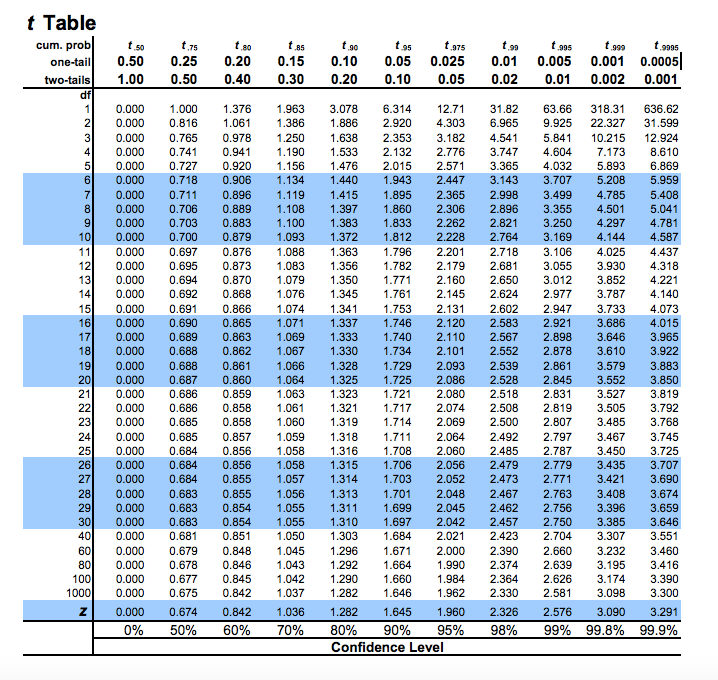
\includegraphics{t_table1z.png}

\url{http://www.sjsu.edu/faculty/gerstman/StatPrimer/t-table.pdf}

\subsection{Alternative t Formula}\label{alternative-t-formula}

\begin{itemize}
\itemsep1pt\parskip0pt\parsep0pt
\item
  Sigma-Hat (estimate of a population standard deviation from sample
  data)

  \begin{itemize}
  \itemsep1pt\parskip0pt\parsep0pt
  \item
    $\hat{\sigma} \sqrt{\frac{\Sigma(x - \bar{x})^2}{n-1}}$ *The t Test
    of Statistical Significance (calculated with sigma-hat
    ($\hat{\sigma}$))
  \item
    $t = \frac{\bar{x}-\mu}{\frac{\hat{\sigma}}{\sqrt{n}}}$ with degrees
    of freedom $df = n-1$ *The t Test of a Statistical Significance
    (calculated with $s$)
  \item
    $t = \frac{\bar{x}-\mu}{\frac{s}{\sqrt{n -1}}}$ with degrees of
    freedom $df = n-1$
  \end{itemize}
\item
  You must know if your \textbf{Standard Deviation} is from a population
  or a sample.
\item
  Consult with the manual of the calculator, computer, or note where the
  standard deviation comes from. It might be a population parameter
  $\sigma$ or a sample statistics $s$.
\item
  You select the \emph{correct} t test based on the standard deviation.
\end{itemize}

\subsection{Z\ldots{}again: A z Test for
Proportions}\label{zagain-a-z-test-for-proportions}

\subsubsection{$z$ test for Proportions}\label{z-test-for-proportions}

This test is designed to test whether the difference between proportions
in a sample reflects the difference in the population.

\subsubsection{Equation: A z Test for
Proportions}\label{equation-a-z-test-for-proportions}

\begin{itemize}
\itemsep1pt\parskip0pt\parsep0pt
\item
  $z = \frac{P_s - P_p}{\sqrt{\frac{P_PQ_p}{n}}}$
\end{itemize}

\subsubsection{What the Symbols Mean}\label{what-the-symbols-mean}

\begin{itemize}
\itemsep1pt\parskip0pt\parsep0pt
\item
  $P_s$ = the proportion in the sample or group
\item
  $P_p$ = the proportion in the population
\item
  $Q_p$ = the proportion of the remaining members in the population

  \begin{itemize}
  \itemsep1pt\parskip0pt\parsep0pt
  \item
    $Q_p = 1-P_p$ because of probabilities (they always add to 1 or
    100\%)
  \end{itemize}
\item
  $n$ = the size of the sample or group being studied
\end{itemize}

\subsection{Example: A z Test for Proportions in
Action}\label{example-a-z-test-for-proportions-in-action}

\subsubsection{Scenario (pg. 253): This is a $z$ Test for
Proportion}\label{scenario-pg.-253-this-is-a-z-test-for-proportion}

In a small community, the \emph{proportions} of minorities make up 20\%
of the population. The School Board President believes that minorities
as teachers are under-represented in a specific school system. The
current number of teachers is 100. Finally, the current system has only
15 minority faculty.

Let:

\begin{itemize}
\itemsep1pt\parskip0pt\parsep0pt
\item
  $P_s$ = .15 (population of minorities in the sample)
\item
  $P_p$ = .20 (the proportion of minorities in the population)
\item
  $Q_p$ = the proportion of the remaining members in the population

  \begin{itemize}
  \itemsep1pt\parskip0pt\parsep0pt
  \item
    $Q_p = 1-P_p$ because of probabilities (they always add to 1 or
    100\%)
  \item
    $Q_p = 1-P_p$ or $1 - .20 = 0.80$
  \end{itemize}
\item
  $n$ = 100 (the size of the sample or group being studied)
\item
  $\alpha = 0.05$ and $z_{crit}=1.65$
\end{itemize}

\subsubsection{Hypothesis}\label{hypothesis-1}

\begin{itemize}
\itemsep1pt\parskip0pt\parsep0pt
\item
  Based on the scenario\ldots{}we can use a one-tailed\ldots{} a
  directional hypothesis
\end{itemize}

$H_0: P_s = P_p$ and $H_1: P_s < P_p$

\subsection{Example: A z Test for Proportions in Action,
continued}\label{example-a-z-test-for-proportions-in-action-continued}

\subsubsection{Scenario (pg. 253): This is a $z$ Test for
Proportion}\label{scenario-pg.-253-this-is-a-z-test-for-proportion-1}

Our equation that we are interested in is:

\begin{itemize}
\item
  $z = \frac{P_s - P_p}{\sqrt{\frac{P_PQ_p}{n}}}$ =
  $\frac{.15 - .20}{\sqrt{\frac{(.20) x (.80)}{100}}}$
\item
  Solving we have $\frac{-.05}{\sqrt{\frac{.16}{100}}}$ =
  $\frac{-.05}{\sqrt{.0016}}$ = $\frac{-.05}{.04}=-1.25$
\item
  Our calculated z score for proportions is: $-1.25$
\end{itemize}

\subsubsection{Decision}\label{decision}

\begin{itemize}
\itemsep1pt\parskip0pt\parsep0pt
\item
  Hypothesis test results: $1.25 < 1.65$
\item
  We fail to reject $H_0$
\item
  We \textbf{cannot} conclude that minorities are underrepresented among
  the teachers.
\end{itemize}

\subsection{Interval Estimation}\label{interval-estimation}

\subsubsection{Interval Estimation:}\label{interval-estimation-1}

\begin{itemize}
\itemsep1pt\parskip0pt\parsep0pt
\item
  An interval of scores that is established, within which a population's
  mean (or another parameter is likely to fall, when that parameter is
  being estimated from sample data).
\end{itemize}

\subsubsection{Confidence Intervals for Means and
Proportions}\label{confidence-intervals-for-means-and-proportions}

\begin{itemize}
\itemsep1pt\parskip0pt\parsep0pt
\item
  An estimated interval within which we are ``confident'' -- based on
  sampling theory -- that the parameter we are trying to estimate will
  fall.
\end{itemize}

\subsection{Confidence Intervals for z
Scores\ldots{}}\label{confidence-intervals-for-z-scores}

\subsubsection{For 95\%:
$\bar{x} \pm 1.96(\frac{\sigma}{\sqrt{n}})$}\label{for-95-barx-pm-1.96fracsigmasqrtn}

\begin{itemize}
\itemsep1pt\parskip0pt\parsep0pt
\item
  GIVEN: $\bar{x}=55$, $\sigma = 10$ and $n=64$
\item
  The UPPER limit would be $55 + 1.96(\frac{10}{\sqrt{64}})$ =
  $55 + 1.96(\frac{10}{8})$ = $55 + 2.45$ = 57.45
\item
  The LOWER limit would be $55 - 1.96(\frac{10}{\sqrt{64}})$ =
  $55 - 1.96(\frac{10}{8})$ = $55 - 2.45$ = 52.55
\item
  The 95\% confidence interval with $\bar{x}=55$, $\sigma = 10$ and
  $n=64$ is (52.55, 57.45).

  \begin{itemize}
  \itemsep1pt\parskip0pt\parsep0pt
  \item
    \textbf{You can write this as: 95\% CI = (52.55, 57.45)}
  \end{itemize}
\end{itemize}

\subsubsection{For 99\%:
$\bar{x} \pm 2.58(\frac{\sigma}{\sqrt{n}})$}\label{for-99-barx-pm-2.58fracsigmasqrtn}

\begin{itemize}
\itemsep1pt\parskip0pt\parsep0pt
\item
  GIVEN: $\bar{x}=55$, $\sigma = 10$ and $n=64$
\item
  The UPPER limit would be $55 + 2.58(\frac{10}{\sqrt{64}})$ =
  $55 + 2.58(\frac{10}{8})$ = $55 + 3.23$ = 58.23
\item
  The LOWER limit would be $55 - 2.58(\frac{10}{\sqrt{64}})$ =
  $55 - 2.58(\frac{10}{8})$ = $55 - 3.23$ = 51.77
\item
  The 99\% confidence interval with $\bar{x}=55$, $\sigma = 10$ and
  $n=64$ is (51.77, 58.23).

  \begin{itemize}
  \itemsep1pt\parskip0pt\parsep0pt
  \item
    \textbf{You can write this as: 99\% CI = (51.77, 58.23)}
  \end{itemize}
\end{itemize}

\subsection{What about the t test confidence
intervals???}\label{what-about-the-t-test-confidence-intervals}

\begin{itemize}
\itemsep1pt\parskip0pt\parsep0pt
\item
  t-Test Confidence Intervals when $\sigma$ is unknown $\hat{\sigma}$
  version

  \begin{itemize}
  \itemsep1pt\parskip0pt\parsep0pt
  \item
    $\mu = \bar{x} \pm t_{critical}(\frac{\hat{\sigma}}{\sqrt{n}})$
  \end{itemize}
\item
  t-Test Confidence Intervals when $\sigma$ is unknown $s$ sample
  version

  \begin{itemize}
  \itemsep1pt\parskip0pt\parsep0pt
  \item
    $\mu = \bar{x} \pm t_{critical}(\frac{s}{\sqrt{n-1}})$
  \end{itemize}
\end{itemize}

\subsubsection{t Test at 95\% Confidence
Intervals}\label{t-test-at-95-confidence-intervals}

\begin{itemize}
\itemsep1pt\parskip0pt\parsep0pt
\item
  Non directional $t_{critical}$
\item
  DF = 1
\item
  $\alpha = 0.05$
\end{itemize}

\subsubsection{t Test at 99\% Confidence
Intervals}\label{t-test-at-99-confidence-intervals}

\begin{itemize}
\itemsep1pt\parskip0pt\parsep0pt
\item
  Non directional $t_{critical}$
\item
  DF = 1
\item
  $\alpha = 0.01$
\end{itemize}

\subsubsection{SPSS DOES THIS FOR YOU.}\label{spss-does-this-for-you.}

Visit
\url{http://academic.udayton.edu/gregelvers/psy216/spss/ttests.htm} for
a tutorial outside of class.

\subsection{Confidence Intervals for
Proportions}\label{confidence-intervals-for-proportions}

\subsubsection{Equation: Confidence Intervals for Proportions using
$z_{critical}$ at
95\%}\label{equation-confidence-intervals-for-proportions-using-zux5fcritical-at-95}

\begin{itemize}
\itemsep1pt\parskip0pt\parsep0pt
\item
  $P_s \pm 1.96(\sqrt{\frac{P_p Q_p}{n}})$
\end{itemize}

\subsubsection{Equation: Confidence Intervals for Proportions using
$z_{critical}$ at
99\%}\label{equation-confidence-intervals-for-proportions-using-zux5fcritical-at-99}

\begin{itemize}
\itemsep1pt\parskip0pt\parsep0pt
\item
  $P_s \pm 2.58(\sqrt{\frac{P_p Q_p}{n}})$
\end{itemize}

\subsection{CI for Proportions an Example at 95\%\ldots{} a
scenario}\label{ci-for-proportions-an-example-at-95-a-scenario}

You are hired as a campaign manager for a local politician in a two
person race. A random stratified telephone survey of 900 likely voters
gives your candidate a 53\% lead over the opponent. How likely does that
percentage lead reflect the outcome electorate? You tell your boss that
you will construct a 95\% confidence interval around the .53 proportion
that your candidate received in the sample.

\subsubsection{That's a lot to comprehend\ldots{}.let's break it
down}\label{thats-a-lot-to-comprehend.lets-break-it-down}

\begin{itemize}
\itemsep1pt\parskip0pt\parsep0pt
\item
  Equation: $P_s \pm 2.58(\sqrt{\frac{P_p Q_p}{n}})$
\end{itemize}

\subsubsection{Given:}\label{given}

\begin{itemize}
\itemsep1pt\parskip0pt\parsep0pt
\item
  $P_s$ = candidate's proportion of support in the sample = .53
\item
  $P_p$ = candidate's proportion of support in the population

  \begin{itemize}
  \itemsep1pt\parskip0pt\parsep0pt
  \item
    estimate or $\hat{P_p}$ \ldots{}. $P_s = P_p = .53$
  \end{itemize}
\item
  $Q_p$ = opponent's proportion of support in the population

  \begin{itemize}
  \itemsep1pt\parskip0pt\parsep0pt
  \item
    $1 - P_p = 1- P_s = 1 - .53 = .47$
  \end{itemize}
\item
  n = number of cases, 900

  \begin{itemize}
  \itemsep1pt\parskip0pt\parsep0pt
  \item
    This is the number of cases, which must equal or exceed
    5/min($P_s 1-P_s$)
  \item
    Really, we say this: 5 divided by whichever is smaller, $P_s$ or
    $1-P_s$
  \end{itemize}
\item
  $\alpha = 0.05$ and $z_{crit}$ = $\pm 1.96$
\end{itemize}

\subsection{CI for Proportions an Example at 95\%\ldots{}
continued}\label{ci-for-proportions-an-example-at-95-continued}

\subsubsection{Upper Limit}\label{upper-limit}

\begin{itemize}
\itemsep1pt\parskip0pt\parsep0pt
\item
  $P_s + 1.96(\sqrt{\frac{P_p Q_p}{n}})$ =
  $.53 +1.96 \sqrt{\frac{(.53)(.47)}{900}}$
\item
  $.53 +1.96 \sqrt{\frac{.2491}{900}}$ = $.53 +1.96 \sqrt{.00028}$ =
  $.53 + 1.96(.0167)$ = $.53 + .0327$ = $.5627$
\end{itemize}

\subsubsection{Lower Limit}\label{lower-limit}

\begin{itemize}
\itemsep1pt\parskip0pt\parsep0pt
\item
  $P_s - 1.96(\sqrt{\frac{P_p Q_p}{n}})$ =
  $.53 -1.96 \sqrt{\frac{(.53)(.47)}{900}}$
\item
  $.53 - 1.96 \sqrt{\frac{.2491}{900}}$ = $.53 -1.96 \sqrt{.00028}$ =
  $.53 - 1.96(.0167)$ = $.53 - .0327$ = $.5027$
\end{itemize}

\subsubsection{CI for the politician: (.5027,
.5627)}\label{ci-for-the-politician-.5027-.5627}

\begin{itemize}
\itemsep1pt\parskip0pt\parsep0pt
\item
  Range is 50\% to 56\%, or 6\% points
\item
  Candidate has a 53\% lead with a margin of error: 3 percentage points
\item
  We could reach 50\% or 56\%
\item
  99\% confidence interval is wider
\item
  n can change the outcome
\end{itemize}

\subsection{A FEW MORE WORDS ON
PROBABILITY}\label{a-few-more-words-on-probability}

Statistical testing is rooted in probability. We have to introduce some
more probability concepts:

\begin{itemize}
\itemsep1pt\parskip0pt\parsep0pt
\item
  P(A)

  \begin{itemize}
  \itemsep1pt\parskip0pt\parsep0pt
  \item
    The probability of outcome A occurring
  \end{itemize}
\item
  P(A or B)

  \begin{itemize}
  \itemsep1pt\parskip0pt\parsep0pt
  \item
    The probability of either outcome A or outcome b occurring
  \end{itemize}
\item
  P(A and B)

  \begin{itemize}
  \itemsep1pt\parskip0pt\parsep0pt
  \item
    The probability of both outcomes A and B occurring jointly
  \end{itemize}
\item
  P(A \textbar{} B) \emph{Baye's Formula}

  \begin{itemize}
  \itemsep1pt\parskip0pt\parsep0pt
  \item
    Conditional probability, that the outcome of A occurring given that
    that outcome B has already occurred.
  \end{itemize}
\end{itemize}

\subsection{Conditional Probability : Addition Rules of
Probability}\label{conditional-probability-addition-rules-of-probability}

\subsubsection{The probability of outcome $A$ occurring given that the
outcome for $B$ has already
occurred.}\label{the-probability-of-outcome-a-occurring-given-that-the-outcome-for-b-has-already-occurred.}

\begin{itemize}
\itemsep1pt\parskip0pt\parsep0pt
\item
  Addition Rules of Probability

  \begin{itemize}
  \itemsep1pt\parskip0pt\parsep0pt
  \item
    A rule by which when outcomes are \textbf{MUTUALLY EXCLUSIVE}, the
    probability of either outcome occurring is the sum of the
    probabilities of each outcome occurring.
  \end{itemize}
\end{itemize}

P(A or B) = P(A) + P(B) for heads/tails on a ``fair'' coin\ldots{}. .50
+ .50 = 1.0

\begin{itemize}
\itemsep1pt\parskip0pt\parsep0pt
\item
  Longer Version: accounting for the interaction between the two
  probabilities.
\end{itemize}

P(A or B) = P(A) + P(B) - P(A and B)

\begin{itemize}
\itemsep1pt\parskip0pt\parsep0pt
\item
  This is important when we are understanding tests of significance
  because we are looking at the probability of something occurring.
\end{itemize}

\subsection{Multiplication Rules of Probability and Statistically
\emph{Independent}
Probability}\label{multiplication-rules-of-probability-and-statistically-independent-probability}

\begin{itemize}
\itemsep1pt\parskip0pt\parsep0pt
\item
  Multiplication Rules of Probability

  \begin{itemize}
  \itemsep1pt\parskip0pt\parsep0pt
  \item
    A rule that is used to find $P(A and D)$.\\
  \item
    P(A and B) = P(A) X P(B)
  \item
    P(A and B and C) = P(A) X P(B) X P(C)
  \end{itemize}
\item
  Statistically Independent P(A \textbar{} B)

  \begin{itemize}
  \itemsep1pt\parskip0pt\parsep0pt
  \item
    P(A \textbar{} B) = P(A)
  \item
    P(B \textbar{} A) = P(B)
  \item
    Return to Multiplication rule: P(A and B)
  \end{itemize}
\end{itemize}

$P(A and B) = P(A) X P(B | A) = P(A) X P(B)$

\subsection{Permutations and
Combinations}\label{permutations-and-combinations}

\begin{itemize}
\itemsep1pt\parskip0pt\parsep0pt
\item
  Permutations

  \begin{itemize}
  \itemsep1pt\parskip0pt\parsep0pt
  \item
    The total possible samples that can be drawn from a population where
    the order of selection is a factor.
  \item
    Permutations $P_K^N = \frac{N!}{(N-K)!}$
  \end{itemize}
\item
  Combinations

  \begin{itemize}
  \itemsep1pt\parskip0pt\parsep0pt
  \item
    The total possible samples when the order of selection is ignored.
  \item
    Combinations $C_K^N = \frac{N!}{K!(N-K)!}$
  \end{itemize}
\item
  What does it mean?

  \begin{itemize}
  \itemsep1pt\parskip0pt\parsep0pt
  \item
    $K$ = the size of the sample to be drawn
  \item
    $N$ = the number of items in the population
  \item
    $N!$ = N factorial $5! = 5 x 4 x 3 x 2 x 1$ and $4! = 4 x 3 x 2 x 1$
  \end{itemize}
\end{itemize}

\subsection{Permutations and Combinations
Examples}\label{permutations-and-combinations-examples}

\subsubsection{Perumtation}\label{perumtation}

\begin{itemize}
\itemsep1pt\parskip0pt\parsep0pt
\item
  Given N = 5 marbles, K = 3 colors (red, blue, green)
\item
  Solve the permutation

  \begin{itemize}
  \itemsep1pt\parskip0pt\parsep0pt
  \item
    $P_K^N = \frac{N!}{(N-K)!}$ = $P_K^N = \frac{5!}{(5-3)!}$ =
    $P_K^N = \frac{5!}{2!}$ = $P_K^N = \frac{5 x 4 x 3 x 2 x 1}{2 x 1}$
    = $\frac{120}{2}$ = $60$
  \end{itemize}
\end{itemize}

\subsubsection{Combination}\label{combination}

\begin{itemize}
\itemsep1pt\parskip0pt\parsep0pt
\item
  Given N = 5 marbles, K = 3 colors (red, blue, green) but the
  \emph{order} matters this time
\item
  Solve the combination

  \begin{itemize}
  \itemsep1pt\parskip0pt\parsep0pt
  \item
    $C_K^N = \frac{N!}{K!(N-K)!}$ = $\frac{5!}{3!(5-3)!}$ =
    $\frac{5!}{3!2!}$ = $\frac{5 x 4 x 3 x 2 x 1}{(3 x 2 x 1)(2 x 1)}$ =
    $\frac{120}{(6)(2)}$ = $\frac{120}{12}$ = $10$
  \end{itemize}
\end{itemize}

\subsection{Review}\label{review}

\subsubsection{We will be coming up on more equations and
techniques\ldots{}if you are
confused}\label{we-will-be-coming-up-on-more-equations-and-techniquesif-you-are-confused}

COME BY MY OFFICE DURING OFFICE HOURS :)

\begin{itemize}
\itemsep1pt\parskip0pt\parsep0pt
\item
  Remember that you can use your text books and notes on an
  exam\ldots{}but you will need to know how to use that efficiently
  during a timed exam.
\end{itemize}

\subsection{Equations}\label{equations}

\begin{itemize}
\itemsep1pt\parskip0pt\parsep0pt
\item
  Z Formula for the Area Under a Standard Normal Curve

  \begin{itemize}
  \itemsep1pt\parskip0pt\parsep0pt
  \item
    $z = \frac{x - \mu}{\sigma}$
  \end{itemize}
\item
  Sigma-Hat (estimate of a population standard deviation from sample
  data)

  \begin{itemize}
  \itemsep1pt\parskip0pt\parsep0pt
  \item
    $\hat{\sigma} \sqrt{\frac{\Sigma(x - \bar{x})^2}{n-1}}$ *The t Test
    of Statistical Significance (calculated with sigma-hat
    ($\hat{\sigma}$))
  \item
    $t = \frac{\bar{x}-\mu}{\frac{\hat{\sigma}}{\sqrt{n}}}$ with degrees
    of freedom $df = n-1$ *The t Test of a Statistical Significance
    (calculated with $s$)
  \item
    $t = \frac{\bar{x}-\mu}{\frac{s}{\sqrt{n -1}}}$ with degrees of
    freedom $df = n-1$
  \end{itemize}
\item
  The z Test for Difference of Proportions
\item
  $z = \frac{P_s - P_p}{\sqrt{\frac{P_PQ_p}{n}}}$
\end{itemize}

\subsection{Equations, continued}\label{equations-continued}

\begin{itemize}
\itemsep1pt\parskip0pt\parsep0pt
\item
  Confidence Intervals for 95\% using $z$

  \begin{itemize}
  \itemsep1pt\parskip0pt\parsep0pt
  \item
    $\bar{x} \pm 1.96(\frac{\sigma}{\sqrt{n}})$
  \end{itemize}
\item
  Confidence Intervals for 99\% using $z$

  \begin{itemize}
  \itemsep1pt\parskip0pt\parsep0pt
  \item
    $\bar{x} \pm 2.58(\frac{\sigma}{\sqrt{n}})$
  \end{itemize}
\item
  Confidence Intervals for Proportions: z 95\%

  \begin{itemize}
  \itemsep1pt\parskip0pt\parsep0pt
  \item
    $P_s \pm 1.96(\sqrt{\frac{P_p Q_p}{n}})$
  \end{itemize}
\item
  Confidence Intervals for Proportions: z 99\%

  \begin{itemize}
  \itemsep1pt\parskip0pt\parsep0pt
  \item
    $P_s \pm 2.58(\sqrt{\frac{P_p Q_p}{n}})$
  \end{itemize}
\item
  t-Test Confidence Intervals when $\sigma$ is unknown $\hat{\sigma}$
  version

  \begin{itemize}
  \itemsep1pt\parskip0pt\parsep0pt
  \item
    $\mu = \bar{x} \pm t_{critical}(\frac{\hat{\sigma}}{\sqrt{n}})$
  \end{itemize}
\item
  t-Test Confidence Intervals when $\sigma$ is unknown $s$ sample
  version

  \begin{itemize}
  \itemsep1pt\parskip0pt\parsep0pt
  \item
    $\mu = \bar{x} \pm t_{critical}(\frac{s}{\sqrt{n-1}})$
  \end{itemize}
\end{itemize}

\subsection{Probability Terms}\label{probability-terms}

\begin{itemize}
\itemsep1pt\parskip0pt\parsep0pt
\item
  P(A)

  \begin{itemize}
  \itemsep1pt\parskip0pt\parsep0pt
  \item
    The probability of outcome A occurring
  \end{itemize}
\item
  P(A or B)

  \begin{itemize}
  \itemsep1pt\parskip0pt\parsep0pt
  \item
    The probability of either outcome A or outcome b occurring
  \end{itemize}
\item
  P(A and B)

  \begin{itemize}
  \itemsep1pt\parskip0pt\parsep0pt
  \item
    The probability of both outcomes A and B occurring jointly
  \end{itemize}
\item
  P(A \textbar{} B) \emph{Baye's Formula}

  \begin{itemize}
  \itemsep1pt\parskip0pt\parsep0pt
  \item
    Conditional probability, that the outcome of A occurring given that
    that outcome B has already occurred.
  \end{itemize}
\end{itemize}

\subsection{Permutation and Combination
Equations}\label{permutation-and-combination-equations}

\begin{itemize}
\item
  Permutations $P_K^N = \frac{N!}{(N-K)!}$
\item
  Combinations $C_K^N = \frac{N!}{K!(N-K)!}$
\end{itemize}

\subsection{Level of Significance for Critical Value of
$z$}\label{level-of-significance-for-critical-value-of-z}

\begin{longtable}[c]{@{}ll@{}}
\toprule\addlinespace
Level of Significance & Critical Value of $z$
\\\addlinespace
\midrule\endhead
.05 & 1.96
\\\addlinespace
.01 & 2.58
\\\addlinespace
.001 & 3.29
\\\addlinespace
\bottomrule
\end{longtable}

\subsection{Upcoming Items}\label{upcoming-items}

\begin{itemize}
\itemsep1pt\parskip0pt\parsep0pt
\item
  Upcoming Items

  \begin{itemize}
  \itemsep1pt\parskip0pt\parsep0pt
  \item
    Homework 2 released Monday 10/6/14 due next week 10/13/14 at
    midnight!
  \item
    Exam 2 10/22
  \item
    Writing Draft 10/29
  \item
    Chapter 9 Two-Sample T-tests
  \end{itemize}
\end{itemize}

\end{document}
